\documentclass[conference]{IEEEtran}
\usepackage{graphicx}
\renewcommand\refname{Referências}
\graphicspath{{.}}

\ifCLASSINFOpdf
  % \usepackage[pdftex]{graphicx}
  % declare the path(s) where your graphic files are
  % \graphicspath{{../pdf/}{../jpeg/}}
  % and their extensions so you won't have to specify these with
  % every instance of \includegraphics
  % \DeclareGraphicsExtensions{.pdf,.jpeg,.png}
\else
  % or other class option (dvipsone, dvipdf, if not using dvips). graphicx
  % will default to the driver specified in the system graphics.cfg if no
  % driver is specified.
  % \usepackage[dvips]{graphicx}
  % declare the path(s) where your graphic files are
  % \graphicspath{{../eps/}}
  % and their extensions so you won't have to specify these with
  % every instance of \includegraphics
  % \DeclareGraphicsExtensions{.eps}
\fi
% graphicx was written by David Carlisle and Sebastian Rahtz. It is
% required if you want graphics, photos, etc. graphicx.sty is already
% installed on most LaTeX systems. The latest version and documentation
% can be obtained at: 
% http://www.ctan.org/pkg/graphicx
% Another good source of documentation is "Using Imported Graphics in
% LaTeX2e" by Keith Reckdahl which can be found at:
% http://www.ctan.org/pkg/epslatex
%
% latex, and pdflatex in dvi mode, support graphics in encapsulated
% postscript (.eps) format. pdflatex in pdf mode supports graphics
% in .pdf, .jpeg, .png and .mps (metapost) formats. Users should ensure
% that all non-photo figures use a vector format (.eps, .pdf, .mps) and
% not a bitmapped formats (.jpeg, .png). The IEEE frowns on bitmapped formats
% which can result in "jaggedy"/blurry rendering of lines and letters as
% well as large increases in file sizes.
%
% You can find documentation about the pdfTeX application at:
% http://www.tug.org/applications/pdftex

\begin{document}
\title{Redes 5G}


% author names and affiliations
% affiliations
\author{\IEEEauthorblockN{Tiago Bem}
\IEEEauthorblockA{ up201504412@fc.up.pt \\
Faculdade de Ciências da Universidade do Porto\\
Departamento de Ciências de Computadores\\
Porto, Portugal}
\and
\IEEEauthorblockN{Miguel Dias}
\IEEEauthorblockA{up201503888@fc.up.pt \\
Faculdade de Ciências da Universidade do Porto\\
Departamento de Ciências de Computadores\\
Porto, Portugal}}


% use for special paper notices
%\IEEEspecialpapernotice{(Invited Paper)}




% make the title area
\maketitle

% As a general rule, do not put math, special symbols or citations
% in the abstract
\begin{abstract}
Nos últimos anos, a tecnologia de 4ª Geração tem-se revelado insuficiente tendo em conta as recentes e crescentes necessidades no campo das tecnologias de comunicação móveis. Isto deve-se ao exponencial crescimento do número de utilizadores de dispositivos que diariamente se interligam através de redes de comunicação sem fios. Este estado de maturação avançado das redes 4G permite antecipar que esta não poderá resolver os problemas anteriormente descritos. \par
Desta forma, torna-se fundamental a existência de um serviço com capacidade muito superior à existente e com velocidades a rondar os Gigabit por segundo. Uma possível solução passaria por um aumento na eficiência espectral e energética, o que levaria a uma mudança no padrão dos sistemas de comunicação sem fios, ao ser introduzida esta nova tecnologia de 5ª Geração. Para isso, é necessário certos requisitos, como a utilização de ondas milimétricas, um sistema com um número massivo de antenas e o poder de enviar informação apenas na direção do terminal. \par
Porém ainda não está bem definido quais as características que efetivamente a nova geração deve adotar, embora existam já umas ideias concensuais e, por conseguinte, novas tecnologias já se encontram em fase de estudo e de avaliação.Neste artigo vamos explorar essas referidas caracteristicas que reúnem concenso e perceber um pouco da sua aplicação. 
\end{abstract}

\begin{IEEEkeywords}
mmWaves, Small Cells, mMIMO, Beamforming.
\end{IEEEkeywords}





% For peer review papers, you can put extra information on the cover
% page as needed:
% \ifCLASSOPTIONpeerreview
% \begin{center} \bfseries EDICS Category: 3-BBND \end{center}
% \fi
%
% For peerreview papers, this IEEEtran command inserts a page break and
% creates the second title. It will be ignored for other modes.
\IEEEpeerreviewmaketitle



\section{Introdução}
Recentemente, tem-se registado um exponencial crescimento da popularidade dos dispositivos móveis, muito devido também ao aumento da capacidade quer de armazenamento, quer de novas features. Este crescimento resulta no igual aumento da procura por tecnologias que possibilitam comunicações móveis, tais como dados móveis e wi-fi. Desta forma, ocorre uma massificação quer de dispositivos, quer de redes móveis, e devido ao seu continuo melhoramento, faz com que as pessoas que ainda não aderiram o venham a fazer num futuro bastante próximo.

\begin{figure}
\centering
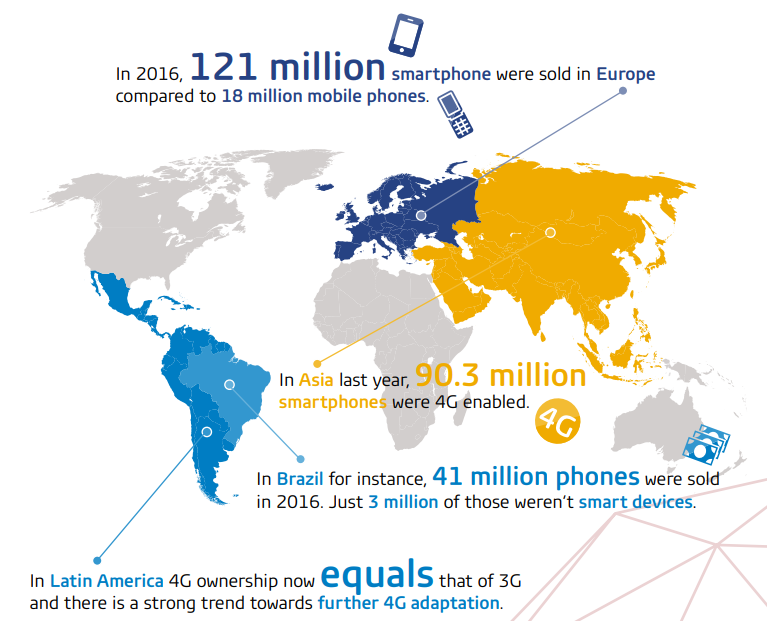
\includegraphics[width=0.9\columnwidth]{IEEEtran/IMG1.png}
\caption{Dados sobre a venda de dispositivos móveis em 2016.[1]}
\end{figure}

O crescimento é notório, de tal forma que se prevê que em 2022 existam 12.3 mil milhões de dispositivos móveis smart para uma população mundial projetada em 8 mil milhões, ou seja, cerca de 1.5 dispositivos per capita [2][3]. Houve um aumento de cerca de 650 milhões de dispositivos móveis em 2017, levando a que atingisse os 8.6 mil milhões comparativamente aos 7.9 mil milhões atingidos em 2015. Espera-se também que em 2022, cerca de três quartos dos dispositivos móveis sejam dispositivos smart, o que, globalmente, representa cerca de 72.8\% do total de dispositivos móveis, comparativamente aos 52.8\% registados em 2017. \par
Ainda neste ano, podemos projetar que a tecnologia 4G representará cerca de 54\% do total de conexões, mas apenas 71\% do tráfego total, ou seja, cerca do dobro de tráfego do que uma rede 3G. Já a tecnologia 5G representará cerca de 3.4\% do total de conexões, mas apenas 11.8\% do tráfego total, o que irá equivaler a 2.6 vezes mais tráfego do que uma rede 4G. Globalmente, o tráfego de dados móveis aumentará sete vezes entre 2017 e 2022, tendo uma taxa de crescimento anual, ou seja, Compound Annual Growth Rate (CAGR) apontada para os 46\%, atingindo assim os 77.5 exabytes por mês até 2022. \par
Até 2022, estes dispostivos gerarão, em média, 6.8GB de tráfego mensal, representando assim o dobro da média de 2017 que se situava nos 3.3GB mensais. Além disso, o tráfego destes irá aumentar 3.5 vezes, atingindo um CAGR de 28\%. \par
Um average smartphone gerará cerca de 11GB de tráfego mensal até 2022, representando um aumento em mais de 4.5 vezes comparativamente aos 2GB mensais de 2017. Até lá, o tráfego agregado destes smartphones será sete vezes maior do que atualmente, situando o CAGR em 48\%. \par
Tudo isto prova que embora muitas características de perfomance desta 5ª Geração estejam asseguradas, a exploração do pouco espectro eletromagnético restante não é o suficiente.
Assim sendo, vejamos agora os requisitos mínimos desta nova tecnologia:

\begin{figure}
\centering
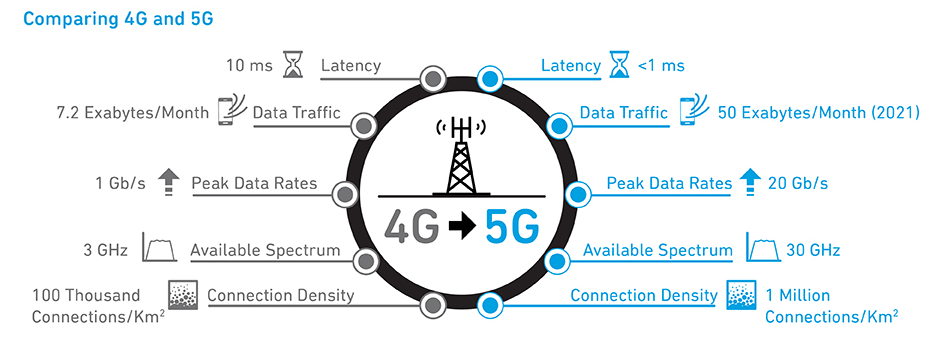
\includegraphics[width=0.99175\columnwidth]{IEEEtran/IMG2.png}
\caption{Comparação entre 4G e 5G[6].}
\end{figure}



\subsection{Gigabit Experience}
Nesta nova tecnologia necessitaremos de experimentar velocidades de receção e transmissão na ordem dos Gigabit por segundo. Por concenso geral determinou-se que a taxa de dados agregados, ou seja a quantidade total que a rede pode suportar, precisará de aumentar em aproximadamente 1000 vezes de 4G para 5G. \par
A taxa de 5\% é a pior taxa de dados que um utilizador pode esperar razoavelmente receber enquanto estiver dentro do alcance da rede. Na quarta geração, as velocidades situavam-se entre 100 Kbps e 1 Gbps. As metas para o 5G relativamente a esta taxa variam de 10 Gbps (o suficiente para suportar streaming de alta definição) a até 100 Gbps. Será um enorme desafio atingir os 10 Gbps para 95\% dos utilizadores, mesmos com grandes avanços tecnológicos, e para tal será necessário um avanço de cerca de 100 vezes em relação ao 4G. Uma vez que estes têm uma taxa tipica de 5\% de aproximadamente 1 Mbps [4]. \par
A taxa de pico é a melhor taxa de dados que um utilizador pode alcançar em qualquer configuração da rede e, embora possa ter uma importância menor do que as taxas anteriores, é importante realçar que se irá situar na faixa das dezenas de Gbps.

\subsection{Zero Latency}
Este termo não significa que não possa existir nenhum atraso, mas sim que os valores de latência serão bastante baixos.
Atualmente, com a tecnologia 4G, estes valores situam-se nos 15ms mas, embora essa latência seja suficiente para a maioria dos serviços atuais, os aplicativos 5G previstos incluem jogos bidirecionais, novas tecnologias baseadas na nuvem, realidade virtual e aprimorada. Dessa forma, torna-se necessário que esta nova tecnologia 5G suporte uma latência na ordem dos 1ms[4].\par
Nesta nova geração, o sistema de comunicações móveis não será apenas utilizado para intereção humana mas também para comunicações de máquinas, por vezes apelidada de "Internet das coisas". Os dispositivos obviamente continuarão a ser controlados remotamente por pessoas, mas agora também se irão comunicar entre si.\par
Assim sendo, a Internet das coisas requer ligações muito mais seguras e confiáveis, e valores de latência bastante mais baixos, pois estas máquinas poderão simplesmente processar informações muito mais rapidamente do que as pessoas[5].

\subsection{Efficiency and coverage}
À medida que avançamos de tecnologia é sempre importante estabelecer um dos objetivos como a diminuição de custos e consumos e energia, embora nem sempre seja isso que aconteça.\par
Porém nesta nova tecnologia 5G é realmente fundamental que esta diminuição aconteça, pois a transmissão de dados será aproximadamente 10 vezes mais rápida e como esta está relacionada com o custo, estima-se que a diminuição se situe nos 90\% comparativamente a 2016. Paralelamente a esta redução de energia que leva consecutivamente à redução de custo, irá haver um significativo aumento da duração da vida das baterias.
Para soluções de baixo rendimento, tais como M2M, as células destas baterias deverão ter uma duração estimada de vida aproxiamadamente 10 vezes superior[6].\par
Uma das razões para se apontar como alvo uma rede significativamente mais eficiente, é o objetivo de que esta tenha uma cobertura bastante maior, de preferência todo o planeta.\par
Desta forma, com a otimização do custo, torna-se possivel a sua implementação em diferentes países, mesmo tendo em conta os diferentes cenários económicos, e torna-se também uma possivel realidade atingir novos locais como aviões, permitindo uma total cobertura da nova geração em relação ao planeta.







\section{Tecnologias chave para o 5G}
O 4G está numa fase em que o suporte já não é atingido e por isso a introdução do 5G torna-se fundamental. Com a rede 5G estão presentes certas caracteristicas que irão ser fundamentais para o desenvolvimento desta nova geração.
\begin{itemize}
    \item Millimeter Waves (mmWaves);
    \item Device-centric architeture;
    \item Massive multiple-in multiple-out (mMIMO);
    \item Beamforming;
\end{itemize}

\subsection{Millimeter Waves (mmWaves)}
Velocidade lenta de internet tem havido sempre e com este fator, um enorme desagrado por parte do utilizador. Assim sendo, uma certa exigência por velocidades de transmissão de dados mais rápidas têm ocorrido, logo, notou-se a necessidade da criação da rede 5G. Millimeter Waves também conhecidas como ondas de frequência extremamente alta, é uma banda de frequências de rádio adequada para redes 5G[7]. \par
Comparada às frequências abaixo de 5 GHz usadas anteriormente por dispositivos móveis, a tecnologia de ondas milimétricas permite a transmissão em frequências entre 30 GHz e 300 GHz[8].
Existem duas maneiras de aumentar a velocidade da transmissão de dados sem fio:
\begin{itemize}
    \item Aumentar a utilização do espectro;
    \item Aumentar a largura de banda do espectro;
\end{itemize}
O uso de ondas milimétricas da 5G usa o segundo dos dois métodos para aumentar as velocidades de transmissão, pois, aumentar a largura de banda do espectro é mais simples e mais direto. Em 2003, a Comissão Federal de Comunicações (FCC) anunciou que as bandas de frequência de 71-76 GHz 81-86 GHz e 92-95 GHz ficaram disponíveis para comunicações de dados de alta velocidade. Este anúncio tornou-se importante porque as redes backbone do 5G passarão de cobre e fibra para mmWaves permitindo rápida afirmação[8].
\begin{figure}[ht]
    \centering
    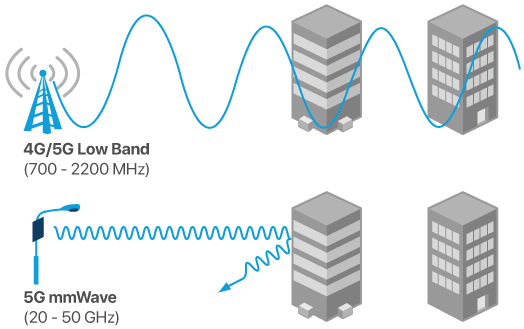
\includegraphics[width=0.9\columnwidth]{IEEEtran/mmwave_diagram.png}
    \caption{Millimeter Waves}
\end{figure}
O uso de frequências de ondas milimétricas pode aumentar facilmente a largura de banda do espectro até 10 vezes, permitindo um aumento muito grande nas velocidades de transmissão[8].\par
No entanto, estas ondas apresentam uma grande desvantagem. Ondas milimétricas são muito suscetíveis a perdas de sinal, bloqueios devido a obstáculos e até mesmo folhas ou chuva podem absorver esses sinais[8]. \par
Como as ondas milimétricas têm altas frequências e comprimentos de onda curtos, as antenas usadas para recebê-las podem ser menores, permitindo a construção de pequenas estações-base. Podemos prever que, no futuro, a comunicação móvel 5G não dependerá mais da construção de estações base em larga escala, mas de muitas pequenas estações base o que permitirá que o 5G cubra áreas periféricas não alcançadas por grandes estações-base[8].\par
Pesquisadores e empresas já têm grandes esperanças em relação à rede 5G, prometendo aos consumidores que esta forneça latência ultra baixa e velocidades de dados sem precedentes[8].

\subsection{Device-centric Architeture}
Device-centric Architeture representa uma mudança de padrão usado no design de futuras tecnologias, pois, com a introdução de redes 5G espera-se melhorar vários serviços enquanto se poupa bastante energia ao fazê-lo. Redes sem fio, que irão usar Device-centric Architeture, devem melhorar significativamente a eficiência energética, a qualidade do serviço, e a capacidade em comparação com as redes atuais. Estão a receber muita atenção devido ao aumento da capacidade de computação, armazenamento e conectividade dos dispositivos móveis. \par
Redes baseadas em Device-centric Architeture defendem a necessidade de explorar e evoluir das arquiteturas atuais, centradas em células, para a arquitetura centrada em dispositivos, um determinado dispositivo deve ter a capacidade de comunicar, através da transação de numerosas informações, usando vários conjuntos de nós[9].\par
Algumas soluções presentes nestas redes são, Device two Device (D2D) e Multiple hop Cellular Networks (MCNs), estas oferecem recursos únicos para superar os limites fundamentais de comunicação e propagação de rádio das arquiteturas tradicionais centradas em células[9].
\begin{figure}[ht]
    \centering
    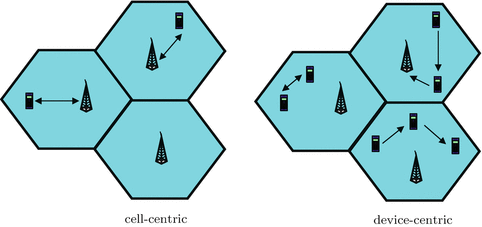
\includegraphics[width=0.9\columnwidth]{IEEEtran/Device-centricArchiteture.png}
    \caption{Device-centric Architeture}
\end{figure}
A ideia é poderem evoluir os dispositivos móveis para passarem a ser nós mais ativos que participam na gestão e operação da infraestrutura celular. Estes smart devices fornecerão conectividade sem fio a outros dispositivos móveis e assim, funcionam como uma “ponte” entre a infraestrutura celular e outros dispositivos ou entre dispositivos, havendo assim transmissões mais eficientes[9].\par
Embora venham melhorar bastante a tecnologia, estas redes não estão livres de desafios, por exemplo, há necessidade de arquiteturas flexíveis centradas no dispositivo, esquemas de seleção de modo em cenários multi-banda e multi-RAT (Radio Access Technologies), processos de descoberta e gestão de pares eficientes e leves, segurança, entre outros[9].

\subsection{Massive MIMO (mMIMO)}
As altas frequências que se esperam usar no 5G impõem restrições adicionais ao design do sistema em termos de bloqueio e atenuação do sinal. É por isso que abordagens com múltiplas antenas tais como, mMIMO (Massive MIMO), tornam-se uma necessidade em futuros padrões de comunicação, pois permitem uma adaptação eficiente dos parâmetros do sinal transmitido para neutralizar os efeitos de canal das ondas milimétricas.\par
A técnica mMIMO(Massive MIMO) está a ocupar uma parte muito importante na pesquisa que se tem feito em relação às redes 5G e espera-se que seja um dos fatores chave nas novas tecnologias. Esta técnica, também chamada de Full Dimension MIMO, HyperMIMO, e ARGOS, usa um grande número de elementos e opera de maneira totalmente coerente e adaptável[10]. \par
O mMIMO adota o conceito original de multiple-input multiple-output e passa para outro nível, em vez de dezenas, usa centenas ou até mesmo milhares de antenas e com um número não tão grande de terminais (dezenas), a transmissão e receção do sinal são mais acentuadas o que traz grandes melhorias no rendimento e eficiência de energia[10]. 
\begin{figure}[ht]
    \centering
    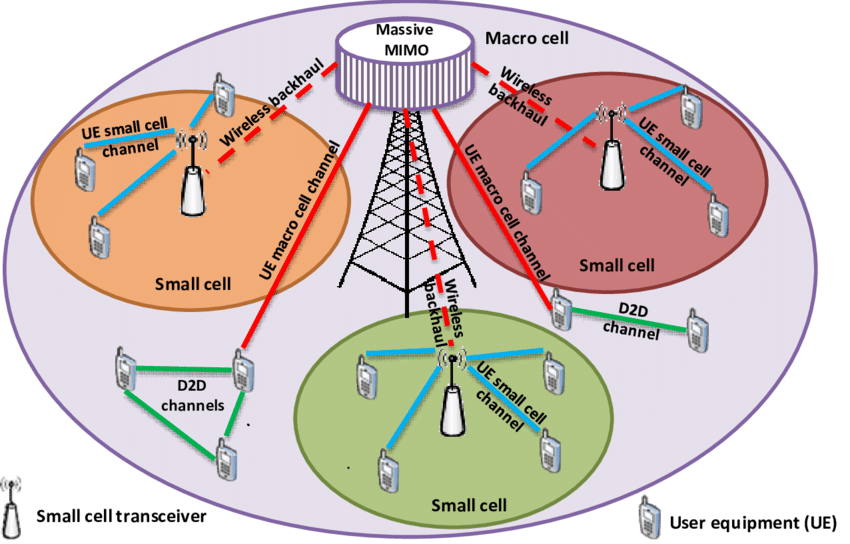
\includegraphics[width=0.9\columnwidth]{IEEEtran/Massive-MIMo.png}
    \caption{Massive MIMO}
\end{figure}
Concretizam o objetivo de aumentar a eficiência espetral do sistema e, fornecer assim, uma qualidade igual de serviço em diferentes ambientes[10].\par
Com a multiplexagem de mensagens para vários dispositivos é esperado um aumento da velocidade em aproximadamente 10 vezes, o pretendido na nova geração[10].

\subsection{Beamforming}
O desenvolvimento da nova geração de comunicações sem fio – 5G – exige requisitos muito mais altos do que a geração anterior (4G) onde, a realização de tais requisitos é algo impossível.\par
Beamforming permite uma comunicação robusta e a nível espectral eficiente, é uma técnica para formar e dirigir um padrão máximo de radiação da antena na direção de interesse[11]. \par
Na rede 5G, este interesse reside em dirigir o padrão máximo de radiação para um determinado equipamento, e assim, maximizar a energia elétrica recebida, atingindo uma diminuição da interferência de sinais nos terminais que permite uma redução da potência de transmissão, capacidade de oferecer altas taxas de dados e possibilidade de estender a cobertura de serviços[11].
\begin{figure}[ht]
    \centering
    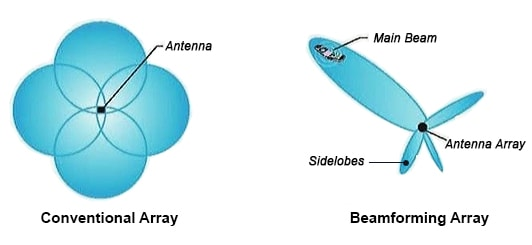
\includegraphics[width=0.9\columnwidth]{IEEEtran/BeamForming.jpg}
    \caption{Beamforming}
\end{figure}
Um dos principais desafios desta técnica será lidar com situações onde se encontra mais do que um utilizador pois uma antena emite na direção pretendida, mas também na direção do terminal que causou interferência[11].



\section{Smarter Devices}
Até agora vimos que a rede 5G será o futuro para a tecnologia móvel. Afinal de contas, vemos que, naturalmente, é o próximo passo a tomar depois do 4G e será com certeza, mais rápida do que qualquer coisa que já tenhamos visto.\par
Vejamos agora, particularmente, o caso de uma smart home. A tecnologia 5G pode revolucionar. Uma smart home é um ambiente onde pode residir um número de pessoas que, além de possuírem computadores e telemóveis (smartphones), também pode conter outros dispositivos como lâmpadas inteligentes, fechaduras inteligentes entre outros dispositivos multifuncionais. Tudo isto, são ótimas maneiras de aperfeiçoar tarefas de casa e não só, porém, também são limitados devido a restrições de velocidade e outros problemas[12].\par
É importante referir que o 5G não é só mais rápido, é muito mais eficiente na maneira como aborda as situações. Oferece menor latência e, portanto, os seus tempos de resposta são mais rápidos e geralmente mais eficientes. Pode lidar com mais usuários simultaneamente do que o 4G devido à capacidade de coexistir com outros sinais sem fio sem riscos de interferência[12]. 
\begin{figure}[ht]
    \centering
    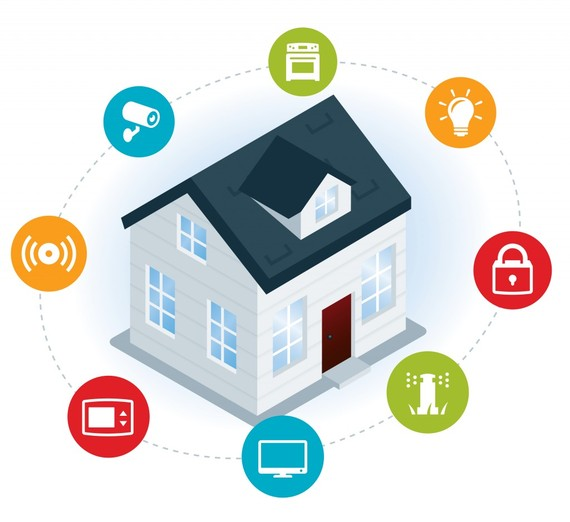
\includegraphics[width=0.6\columnwidth]{IEEEtran/Smart-Home-Ecosystems-2.jpg}
    \caption{Smart Home}
\end{figure}
Smart Home é uma das aplicações mais populares no contexto de IoT (Internet of Things), pois apresenta requisitos bastante desafiantes em termos de performance, segurança e custo.  Até agora, tudo o que se espera atingir com a rede 5G ainda está bastante primitivo, no entanto, o desenvolvimento de aplicações e dispositivos neste contexto está cada vez mais a aumentar. \par
Por último, mas não menos importante, irão ser iniciadas atividades com oportunidades de negócio  para a promoção de 5G Smart Home[12].


\section{Conclusão}
Graças ao constante desenvolvimento e avanço da tecnologia, as infraestruturas de rede móvel têm de igual de forma, vindo a ser renovadas, pois as novas são obviamente bem mais potentes e eficazes do que as precedentes. A primeira geração (1980) era apenas destinada a chamadas de voz, com velocidade na ordem dos 2.4 Kbps, enquanto que na segunda geração (1990) incluia também mensagens de texto e velocidades de 64 Kbps por segundo. Já a terceira geração (2000), atingiu velocidades de 384 Kbps e desta vez, a grande novidade era o acesso a internet através de dados móveis. Com a quarta geração chegou a banda larga móvel, com velocidades entre os 100 Kbps e os 1 Gbps. Nesta nova geração, a 5G, é expectável atingir valores 100 vezes maiores que a anterior tecnologia, com velocidades situados entre os 10 Gbps e 100 Gbps. Um dos principais objetivos para o desenvolvimento desta nova tecnologia é não só a aplicação às comunicações móveis, mas também a implementação em muitas áreas do quotidiano e a promoção de outros avanços tecnológicos, tais como nos carros autónomos.\par
Apesar de todas estas vantagens enumeradas, com esta nova rede 5G advêm novos desafios para os fabricantes de dispositivos sem fios e também para empresas de telecomunicações. Um dos primeiros desafios, situa-se na uniformização da rede, pois espera-se que esta seja flexível e potente o suficiente para surgirem novos serviços. Desta forma, o 5G deverá funcionar em várias faixas eletromagnéticas e funcionar também de igual forma em áreas menos povoadas e/ou rurais e em aparelhos mais avançados. No fundo será o maior desafio desta nova tecnologia, visto que existem ainda, em vários países como Portugal, áreas pouquissimo evoluídas neste campo, pois nem sequer são abrangidas pelo 4G, uma década depois da sua criação. Outro grande desafio, embora não abordado, será definitivamente a segurança, definindo-se assim a maior parte dos seus problemas solucionáveis tanto a nível de software como a nível de hardware.\par
A rede 5G vai claramente revolucionar o mercado e será uma combinação de diversas tecnologias aprimoradas com tecnologia verde, o que permitirá estabelecer uma rede bem mais eficiente com maior capacidade, melhor QoS e ainda possibilitará a sua evolução num futuro quando esta for aperfeiçoada. Falamos claramente, de uma rede muito mais densa e onde o principal alvo é não só a interação humana, mas sim a comunicação Machine-to-Machine (M2M), também chamada de "Internet of Things" (IoT). \par
Esta nova tecnologia já começou a ser implementada em diversos países, tais como em Portugal. A primeira e unica cidade do nosso pais a ter cobertura total de rede 5G foi Matosinhos[13]. Porém muitos países ainda estão em fases de teste e prevê-se que ao longo desta nova década, seja exponencial o número de paises nos quais já se utiliza o 5G. Contudo, nunca saberemos o que o futuro nos reserva e com este enorme avanço tecnológico proporcionado pelo 5G, os investigadores já se começam a questionar se realmente esta tecnologia será auto-suficiente para os próximos anos ou se será realmente necessário começar a pensar em algo cada vez mais evoluído. Será que em 2030 teremos uma nova rede 6G?


\begin{thebibliography}{13}
\bibitem{Ref1} 
Growth from Knowledge:
"Tech Trends 2017: Why 5G is one of the biggest mobile technology trends.",
infographic at gfk.com/insights, Dec.2017

\bibitem{Ref2}
United Nations:
World Population Prospects 2017,
data query at population.un.org/wpp/DataQuery, Dec.2017

\bibitem{Ref3}
Cisco Visual Networking Index:
Global Mobile Data Traffic Forecast Update, 2017-2022,
white paper at Cisco.com, 2019

\bibitem{Ref4}
J.G.Andrews, S.Buzzi, W.Choi, S.Hanly, A.Lozano,
A.C.K. Soong and J.C.Zhang,
"What Will 5G Be?" IEEE Journal on selected areas in communications,
no.6, Jun.2014

\bibitem{Ref5}
Nokia:
"5G use cases and requirements",
white paper at Nokia.com, 2016

\bibitem{Ref6}
Halid Hrasnica and Eurescom GmbH,
"Strategic Research and Innovation Agenda - Version 2",
white paper at networld2020.eu, 2014

\bibitem{Ref7}
Alibaba Clouder,
"Understanding How Millimeter Waves Power the 5G Network",
at alibabacloud.com, Jul.2019

\bibitem{Ref8}
Raed Shubair and Fatima Al-Ogaili,
"Millimeter-Wave Mobile Communications for 5G: Challenges and Opportunities", conference paper, Jun.2016

\bibitem{Ref9}
J.Gozalvez and Baldomero Coll-Perales,
"Device-Centric Wireless Networks for 5G", conference paper, Sep.2015

\bibitem{Ref10}
Hilal El Misilmani and Ahmad El Hajj,
"Massive MIMO Design for 5G Networks: An Overview on Alternative Antenna Configurations and Channel Model Challenges",
conference paper, Jul.2017

\bibitem{Ref11}
Irina Stepanets, Grigoriy Fokin and Andreas Müller,
"Beamforming Techniques Performance Evaluation for 5G massive MIMO Systems ",
article, Mar.2019

\bibitem{Ref12}
Bruno Dzogovic, Bernardo Santos, Josef Noll, Van Thuan Do,
Boning Feng and Thanh van Do,
"Enabling Smart Home with 5G Network Slicing," 2019 IEEE 4th International Conference on Computer and Communication Systems (ICCCS), Singapore, Feb.2019

\bibitem{Ref13}
Jornal de Notícias,
"Matosinhos é a primeira cidade 5G em Portugal",
at jn.pt, Out.2019

\end{thebibliography}

\end{document}


